\begin{frame}[fragile]
\frametitle{Monte-Carlo Simulation}
\newcommand{\newfilename}{py-MonteCarlo.py}
\begin{itemize}
\item Monte-Carlo simulation to calculate the value of $\pi$
\item The code below shows a straightforward implementation.
\lstinputlisting[language=Python, firstline=20, lastline=30]{../py-MonteCarlo.py}
\end{itemize}
file: \newfilename
\end{frame}

\begin{frame}[fragile]
\frametitle{Monte-Carlo Simulation}
\newcommand{\newfilename}{py-MonteCarlo.py}
\begin{itemize}
\item With Numba jit
\lstinputlisting[language=Python, firstline=3, lastline=14]{../py-MonteCarlo.py}
\end{itemize}
file: \newfilename
\end{frame}

\begin{frame}[fragile]
\frametitle{Monte-Carlo Simulation}
\begin{itemize}
\item Computation time Numba vs Normal script
\begin{figure}
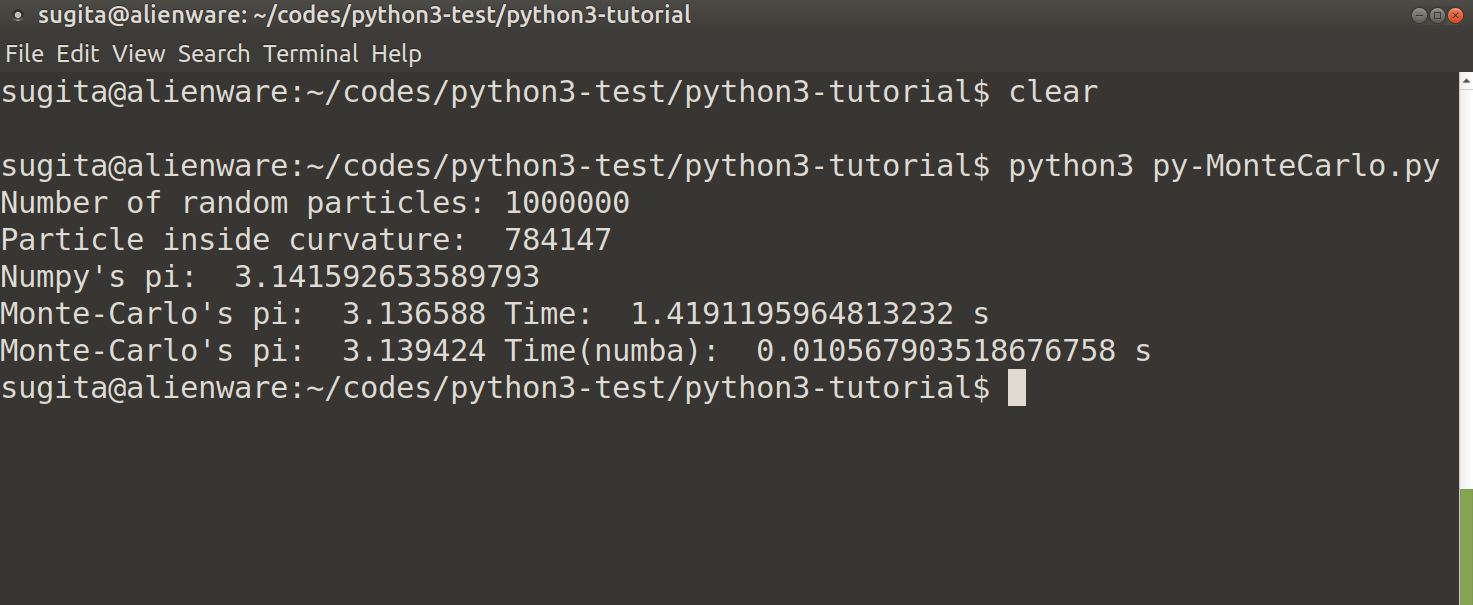
\includegraphics[width=\textwidth]{numba-vs-normal.png}
\caption{Numba vs normal script computation time.}
\end{figure}
\end{itemize}
\end{frame}